\documentclass[a4paper,titlepage]{article}

\usepackage[utf8]{inputenc} % Para poder escribir acentos directamente
\usepackage[spanish]{babel} % Para que el LaTeX sepa que el texto está en español y divida las sílabas al final de una línea correctamente, entre otras cosas
\usepackage[left=3cm, right=3cm, top=3cm, bottom=3cm]{geometry} % Para ajustar los márgenes, ya que por defecto son mayores
\usepackage{graphicx} % Para insertar imágenes

\usepackage{fancyhdr}
\pagestyle{fancy}
\fancyhf{}
\fancyhead[L]{\textbf{Unai Martinez Corral}} % Páginas pares e impares, alineado a la izquierda en la cabecera
\fancyhead[R]{unai.martinez@udc.es} % Páginas pares e impares, alineado a la derecha en la cabecera
\fancyfoot[C]{\textbf{Universidade da Coruña}} % Páginas pares e impares, centrado en el pie
\fancyfoot[L]{EUP Ferrol} % Páginas pares e impares, alineado a la izquierda en el pie
\fancyfoot[R]{2009/2010} % Páginas pares e impares, alineado a la derecha en el pie
\renewcommand{\footrulewidth}{0.4pt}

%--------------------------------------------------------------------------

\begin{document}

\begin{center}
\LARGE{\textbf{Tecnología Electrónica}}\\
\LARGE{Amplificador de instrumentación}
\end{center}

%--------------------------------------------------------------------------

El amplificador de instrumentación es un dispositivo creado a partir de amplificadores operacionales diseñado para tener una alta impedancia de entrada y un alto rechazo al modo común (CMRR).
El término 'rechazo al modo común' hace referencia a un parámetro de los amplificadores operacionales. En el montaje que vamos a analizar, cuando las tensiones en las patillas $V^{+}$ y $V^{-}$ son iguales,
existe una pequeña señal de salida. Lo ideal sería que ésta fuera cero. De ahí la importancia del alto rechazo, pues garantiza que dicha señal será lo más pequeña posible.

\begin{figure}[!ht]
 \begin{center}
  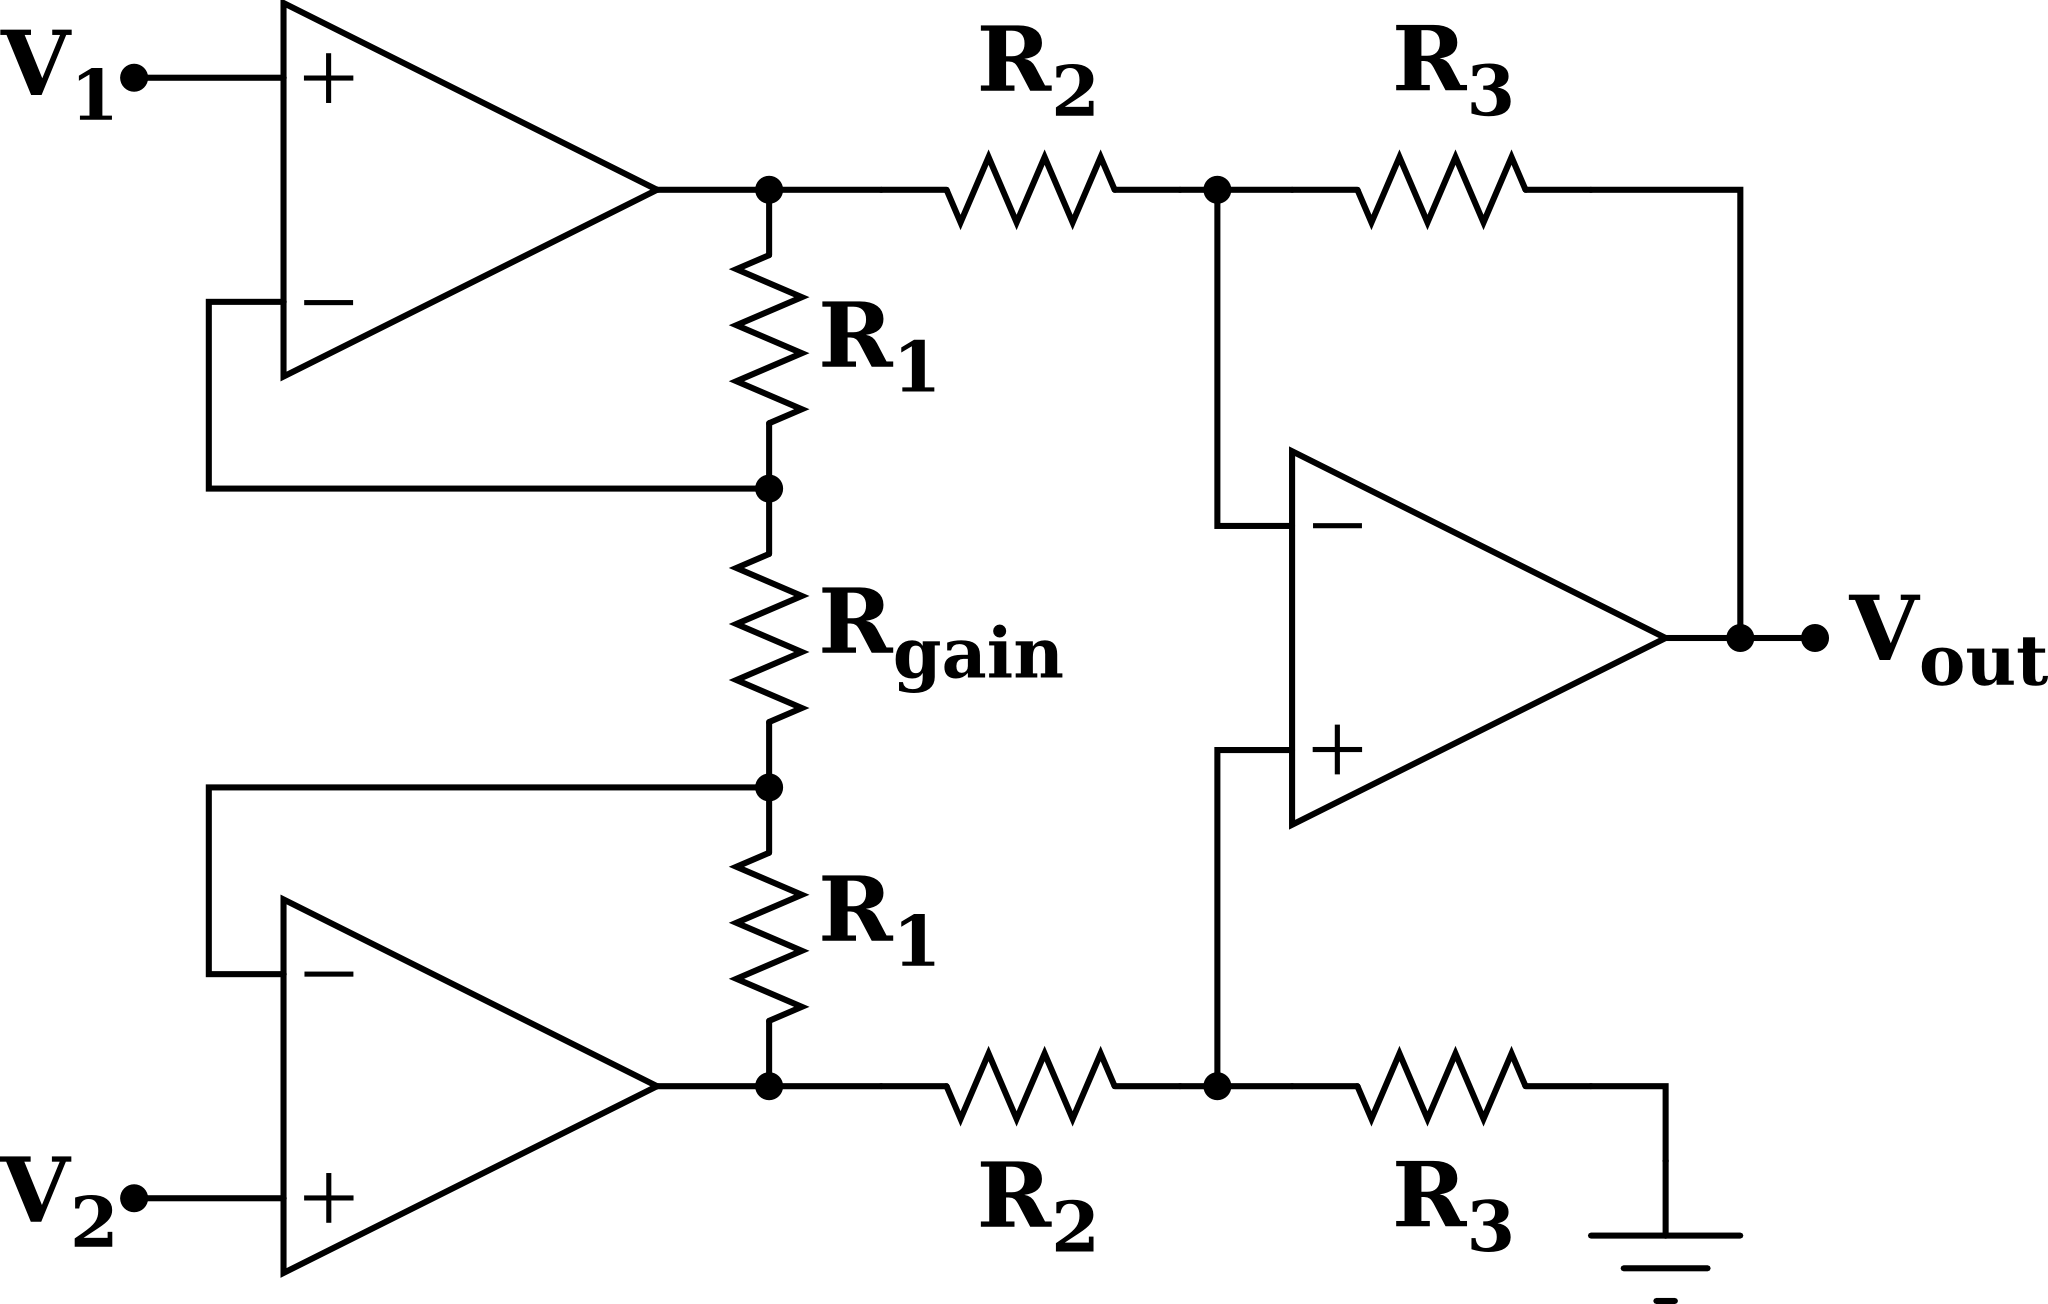
\includegraphics[width=260pt]{./Opampinstrumentation.png}
  \caption{Amplificador de instrumentacion construido con componentes discretos}
  \label{AO_inst}
 \end{center}
\end{figure}

Se trata de un dispositivo disponible en diversos encapsulados, como por ejemplo el INA114 que fabrica la empresa Burr-Brown en formato DIP-8 y SOL-16. Sin embargo, el análisis de este tipo de dispositivos no
resulta de interés para la labor que nos ocupa, pues el objetivo es analizar el funcionamiento interno de éste y no sus posibles aplicaciones. En este sentido, la Figura~\ref{AO_inst} muestra la configuración
interna de un amplificador de instrumentación estándar. Como puede observarse, está compuesto por tres amplificadores operacionales y un total de cinco resistencias con tres valores diferentes. La entrada está
compuesta por dos tensiones y obtenemos una sola como salida. A fin de entender mejor el análisis del dispositivo, lo dividiremos en dos etapas. La primera de ellas la compondrán los dos amplificadores operacionales
situados a la izquierda, cuyas salidas son las entradas del tercero. A partir de los valores obtenidos para las salidas, solucionaremos la etapa de la derecha, que como veremos no es mas que un montaje restador.

\begin{figure}[!h]
 \begin{center}
  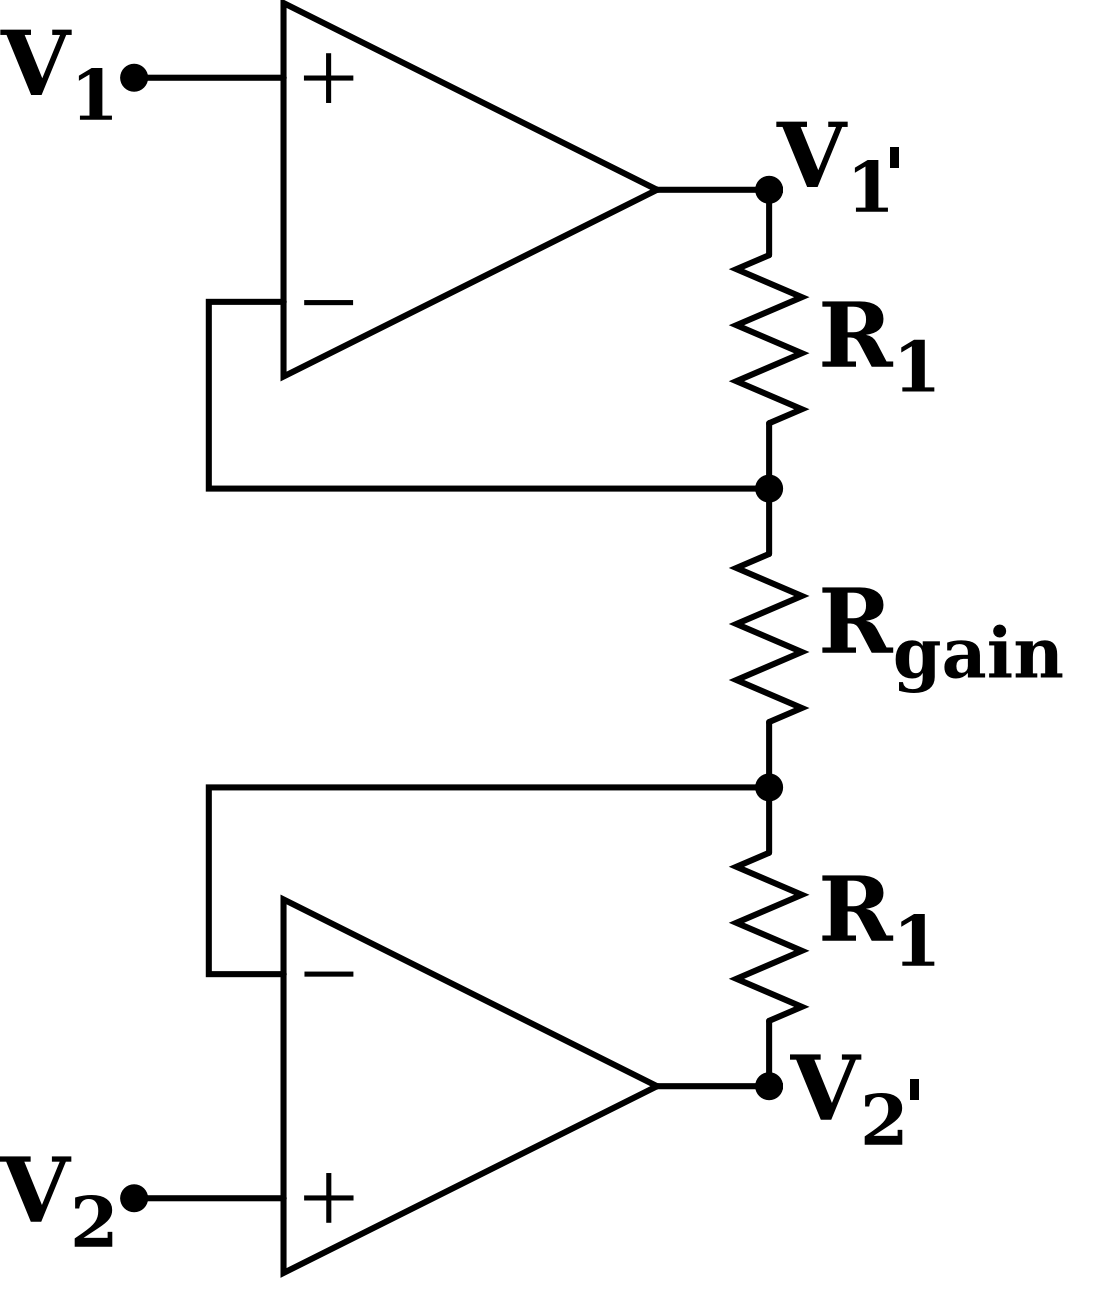
\includegraphics[width=130pt]{./parte1.png}
  \caption{Tratamiento de las tensiones de entrada}
  \label{Parte1}
 \end{center}
\end{figure}

Podemos ver en la Figura~\ref{Parte1} que el tratamiento de las tensiones consiste en un montaje formado por dos amplificadores operacionales y tres resistencias. Para calcular los valores de $V_{1'}$ y $V_{2'}$, debemos
tener en cuenta dos caracteristicas básicas de los amplificadores operacionales. La primera de ellas es que la impedancia de entrada es idealmente infinita. No sucede lo mismo con la salida, pero como veremos, esto
no nos afecta. En segundo lugar, el concepto de 'masa virtual' nos indica que la tensión en la patilla $V^{+}$ de un amplificador es igual a la que encontramos en la patilla $V^{-}$. Teniendo esto en cuenta, podemos
saber que la tensión existente en el punto común entre $R_{gain}$ y la resistencia $R_{1}$ de la parte superior es $V_{1}$, y la que tenemos entre $R_{gain}$ y la resistencia $R_{1}$ de la parte inferior $V_{2}$.

Hechas las valoraciones anteriores, conocemos la tensión existente en bornes de $R_{gain}$. Aplicando la Ley de Ohm, podemos calcular la corriente que circula a través de ésta. Además, debido a la impedancia
de entrada infinita, y aplicando la Ley de corrientes de Kirchhoff, sabemos que ésa será la misma corriente que circule a través de las dos resistencias $R_{1}$, por lo que podemos deducir las tensiones $V_{1'}$ y $V_{2'}$.
La corriente que circule desde la salida de cada uno de los operacionales hacia la etapa siguiente nos es indiferente, pues no afecta a la rama que estamos analizando, y por lo tanto no modifica los valores de las
tensiones a calcular:

\begin{equation}
I_{R_{gain}} = {{(V_{1} - V_{2})} \over {R_{gain}}}
\label{Rgain}
\end{equation}

\begin{equation}
I_{R_{gain}} = I_{R_{1}}
\label{Corrientes}
\end{equation}

\begin{equation}
V_{1'} = V_1 + I_{R_{1}} \cdot R_1 = V_1 + {{(V_{1} - V_{2})} \over {R_{gain}}} \cdot {R_1}
\label{V1'}
\end{equation}

\begin{equation}
V_{2'} = V_2 - I_{R_{1}} \cdot R_1 = V_2 - {{(V_{1} - V_{2})} \over {R_{gain}}} \cdot {R_1}
\label{V2'}
\end{equation}

Como ya hemos adelantado, la segunda parte del dispositivo es un circuito diferencial o restador compuesto por un amplificador operacional y dos entradas (las salidas de la etapa anterior). La Figura~\ref{Parte2}
muestra esta etapa, con los elementos de la primera ya retirados. El cálculo de este apartado podríamos atacarlo mediante la Ley de corrientes de Kirchhoff y la Ley de Ohm, como hiciéramos en el anterior.
Sin embargo, lo haremos por superposición, dado que mediante este método los circuitos resultantes son ya conocidos y podemos aplicar las fórmulas directamente.

\begin{figure}[!h]
 \begin{center}
  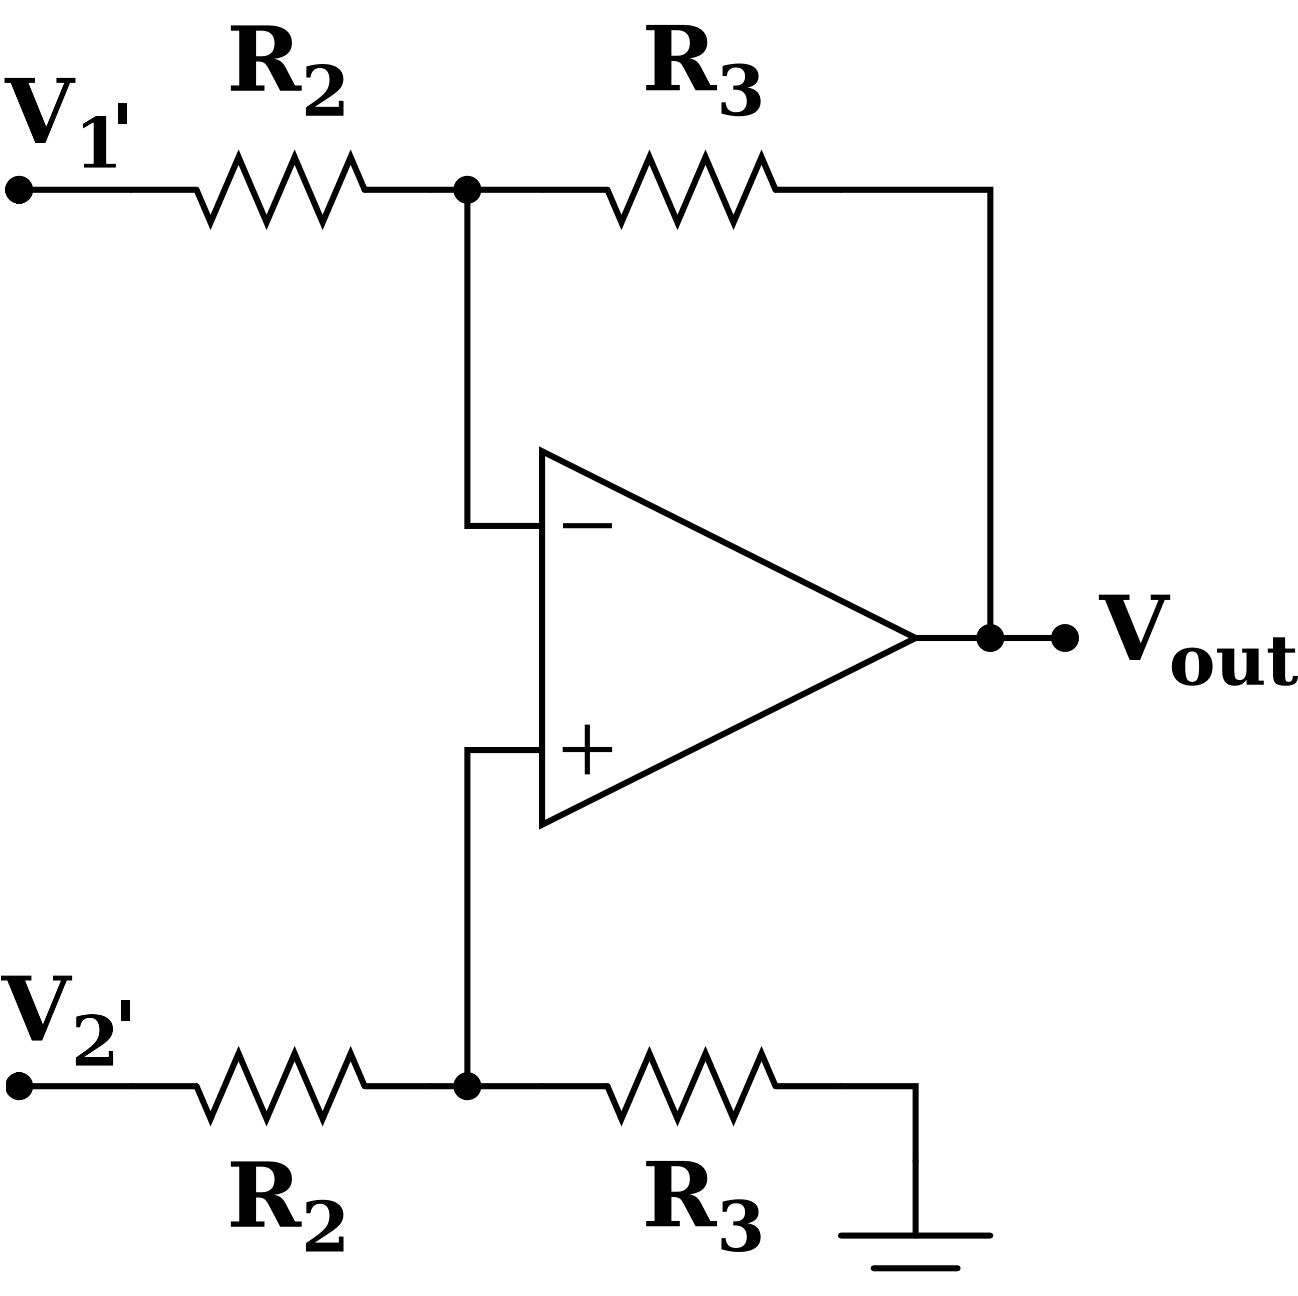
\includegraphics[width=130pt]{./parte2.png}
  \caption{Resto de las señales de entrada modificadas}
  \label{Parte2}
 \end{center}
\end{figure}

En primer lugar dejaremos únicamente la entrada $V_{1'}$, sustituyendo $V_{2'}$ por un cortocircuito. En estas condiciones, la patilla $V^{+}$ del amplificador operacional queda conectada a masa, pues tenemos un divisor
de tensión de masa a masa. El circuito resultante es un montaje inversor. A continuación, sustituiremos $V_{1'}$ por un cortocircuito y nos quedaremos sólo con $V_{2'}$. El resultado es un montaje no inversor, cuya fórmula también nos es conocida:

\begin{equation}
V_{out_1} = - V_{in} \cdot {R_f \over R_{in}} = - V_{1'} \cdot {R_3 \over R_2}
\label{Vout1}
\end{equation}

\begin{equation}
V_{out_2} = V^{+} \cdot (1 + {R_f \over R_{in}}) = V_{2'} \cdot {R_3 \over {R_2 + R_3}} \cdot (1 + {R_3 \over R_2})
\label{Vout2}
\end{equation}

Por último, sumamos las expresiones (\ref{Vout1}) y (\ref{Vout2}) para obtener como resultado el valor final de $V_{out}$:

\begin{equation}
V_{out} = V_{out_1} + V_{out_2} = - V_{1'} \cdot {R_3 \over R_2} + V_{2'} \cdot {R_3 \over {R_2 + R_3}} \cdot (1 + {R_3 \over R_2})
\label{Vout}
\end{equation}

Si quisiéramos la expresión final en funcion de $V_1$ y $V_2$, sólo tendríamos que sustituir (\ref{V1'}) y (\ref{V2'}) en (\ref{Vout}). Pese a que no resulta una sustitución complicada, no he conseguido obtener
los resultados vistos en las fuentes consultadas, por lo que he optado por no desarrollar la expresión:

\begin{equation}
V_{out} = - ({V_1 + {{(V_{1} - V_{2}) \cdot {R_1}} \over {R_{gain}}} }) \cdot {R_3 \over R_2} + ({V_2 - {{(V_{1} - V_{2}) \cdot {R_1}} \over {R_{gain}}} }) \cdot {R_3 \over {R_2 + R_3}} \cdot (1 + {R_3 \over R_2})
\label{Vout_fin}
\end{equation}

\vspace{12cm}

\section*{Referencias}

\begin{itemize}
\item{Wikipedia. Colaboradores de la wikipedia.\\
\small{http://es.wikipedia.org/wiki/Amplificador\_de\_instrumentación} \\
\small{http://es.wikipedia.org/wiki/Rechazo\_al\_modo\_común}}

\item{Instrumentación electrónica de comunicaciones. Tema III. Escuela Ténica Superior de Ingenieros Industriales y de Telecomunicación. Universidad de Cantabria.\\
\small{http://www.ctr.unican.es/asignaturas/instrumentacion\_5\_IT/IEC\_3.pdf}}

\item{Datasheet INA114. Burr-Brown. \\
\small{http://www.datasheetcatalog.org/datasheet/texasinstruments/ina114.pdf}}
\end{itemize}

\end{document}